%% Dieser Quelltext ist in der Kodierung UTF-8 zu speichern und mit lualatex
%% zu kompilieren.

% !TeX program = lualatex

\documentclass{scrartcl}  % KOMA-Scritp equivalent to \documentclass{article}
% \documentclass[12pt,a4paper]{article}
% \usepackage[utf8]{inputenc}
% TODO: fix \setdefaultlanguage problem while compiling
% \setdefaultlanguage[spelling=new, babelshorthands=true]{german}  
\usepackage{polyglossia}  % for LuaLatex
\usepackage{fontspec}  % for LuaLatex
\usepackage{luacode}  % for LuaLatex
\renewcommand{\familydefault}{\sfdefault}  % change serif (default-value) to SansSerif version of LaTex-font
\usepackage{amsmath}  % recommended as an adjunct to serious mathematical typesetting
\usepackage{amsfonts}  % extended set of fonts for use in mathematics
\usepackage{amssymb}  % allows the use of various special characters and symbols
\usepackage{graphicx}  % providing interface for optional arguments to the \includegraphics command
\usepackage{array}  % extended implementation of the array and tabular environments
\usepackage[table]{xcolor}  % for coloring rows in tables, load before \usepackage{xcolor}!!!
\usepackage{xcolor}  % to use broader color plate
\usepackage{hyperref} % to create hypertext links in PDF (jump from content overview to according pages)
\usepackage{enumitem} % for enumerate with letters
\usepackage{textcomp} % for copyright symbol
\usepackage{tcolorbox} % for making boxes around stuff
\usepackage{wrapfig}  % to wrap images and text
\usepackage{lipsum}  % generates filler text
\usepackage{pdflscape}  % for using landscape format in between
\usepackage{smartdiagram}  % to create cooler diagrams
\usepackage{floatrow}  % provides many ways to customize layouts of floating environments
\usepackage{caption}  % for more formating options for captions
\usepackage{gensymb}  % to use symbols
\usepackage{siunitx}  % to use symbols and units
\usepackage[scale=1.5]{ccicons}  % for Creative Commons icons
\usepackage{tikz}  % use for spiderweb diagram
\usepackage{pdfpages}  % include external PDFs

% needed for chemistry notations
\usepackage{chemmacros}  % used for chemistry stuff
\usepackage{chemfig}  % used for chemistry stuff
\usepackage[version=4]{mhchem}   % used for chemistry stuff
\usepackage{modiagram}  % to draw AO (atom orbitals) and MO diagrams
\usepackage{bohr}  % to draw BOHR modells of atoms (till Element 112)
\usepackage{elements}  % collection of data of elements (till Element 112)

% TODO: pst-labo works in pdflatex but not lualatex...work out, wthat and how to fix
% pstricks  
%\usepackage{auto-pst-pdf}
%\usepackage{pst-labo}


% libraries
\tcbuselibrary{skins}  % for textcolorbox
\usetikzlibrary{shapes}


% page layout for worksheets
\usepackage[left=1.50cm, right=1.50cm, top=2.00cm, bottom=2.00cm]{geometry}
\usepackage[headsepline,footsepline]{scrlayer-scrpage}
%scrpage2
\pagestyle{scrheadings}
\setlength{\parindent}{0pt}  % no indentation of paragraphs

% this luacode has no function, except to make sure the document is compiled using LuaLaTex
\begin{luacode*}
	--[[
		print("this is just a comment")
	--]]
\end{luacode*}


% Information for Header and Footer
% *********************************

\ihead{Chemie}
\chead{\textbf{Zombie School}}
\ohead{2021}
% \ohead{90min}
% \ifoot{Fußzeile innen}
\cfoot{\textsf{\pagemark}}
%\ofoot{Fußzeile außen}


\author{Jonas Pews}
\title{Zombie School - Mission 1: Benzinherstellung}
\date{\today}

% Some Info about this document
% *****************************
%
% TODO: write Text how this doc can be used in school. also about RLP Brandenburg/Berlin

% TODO: write more comments to explain/comment :-) the Tex-Code 

% Info for tabing in tex file
% ***************************
% part/section is one tab
% subsection is two tab
% pagebreak/layout changes (landscape) always no tab

\begin{document}

	\begin{center}
		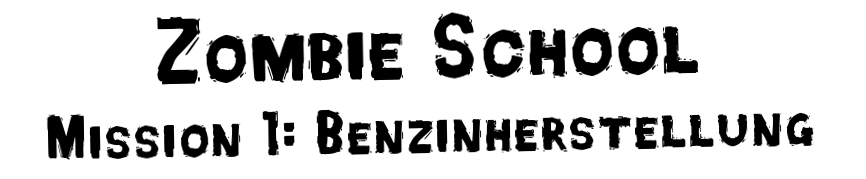
\includegraphics{img/headline_ch_01_raffinerie}
	\end{center}	
	
	\begin{center}
		{\LARGE \textbf{Stelle Treibstoff für ein Fluchtfahrzeug her!}}
	\end{center}
	
\vspace{0.7cm}	
	\textit{Auf dem Parkplatz der Schule steht ein Auto. Du hast nachgesehen und Glück im Unglück: der Schlüssel steckt, der Tank ist leer. Wo der Besitzer ist, willst du gar nicht wissen. Zeit das Auto flott zu kriegen und abzuhauen. Irgendwie musst du also aus den Chemiekalien in der Schule Treibstoff herstellen. Das kann ja nicht so schwer sein.} \newline

\vspace{0.7cm}	

	\textbf{Ziel: Finde heraus, wie man Treibstoff überhaupt herstellt.}
	\begin{enumerate}
		\item Lies dir die einzelnen Texte durch und beantworte dazu die gegebenen Fragen.
		\item Erkläre deiner Lehrkraft am Ende, wie du im Labor Treibstoff herstellen kannst.
	\end{enumerate}

\vspace{0.7cm}	
	\begin{minipage}{0.7\textwidth}
		\noindent \textbf{Am Ende dieses Kapitels sollst du ... :}
		\begin{enumerate}
			\item ... die Unterschiede zwischen dem Stoffgemisch Erdöl und seinen Bestandteilen erklären können.
			\item ... die Bedeutung der Rohstoffe Erdöl und Erdgas erklären können.
			\item ... die Gewinnung der Rohstoffe Erdöl und Erdgas erläutern können.
			\item ... eine Abbildung zum Versuchsaufbau der fraktionierten Destiallation zu beschriften.
			\item ... die Methode der fraktionierten Destillation zur Trennung des Stoffgemisches Erdöl in seine Bestandteile erklären können.
		\end{enumerate}
		\textbf{Vorgehensweise:}
		\begin{enumerate}
			\item Entweder du arbeitest allein, oder du findest eine(n) MitschülerIn.
			\item Wenn ihr als Paar arbeitet, teilt euch die beiden Texte auf und bearbeitet sie getrennt.
			\item Wenn ihr beide fertig seit, tauscht eure Ergebnisse aus und bearbeitet dann die letzte Aufgabe.
		\end{enumerate}
			
	\end{minipage}
	\hspace{0.1\textwidth}
	\begin{minipage}{0.2\textwidth}
		\begin{tcolorbox}
			[enhanced,
			width=0.9\textwidth,
			colback=white,
			colframe=black,
			fonttitle=\sffamily\bfseries\large, 
			title=Zeit,  % search keyword::Zeit
			attach boxed title to top center={xshift=-0.0mm,yshift=-0.50mm},
			boxed title style={skin=enhancedfirst jigsaw,size=small,arc=1mm,bottom=-1mm,colframe=black,height=0.75cm},
			colbacktitle=black,
			drop lifted shadow]
			\centering
			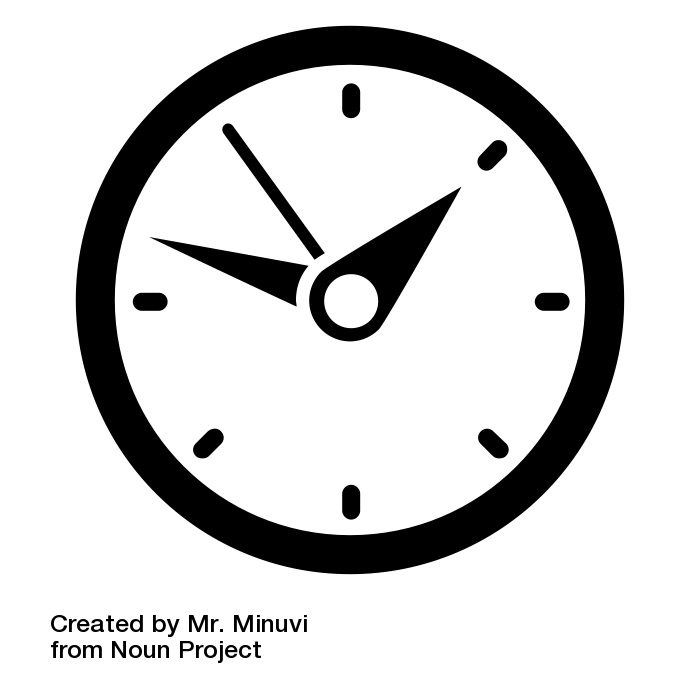
\includegraphics[width=0.9\textwidth]{../symbols/symbol_tex_time}
			
			\begin{center}
				\textbf{90min}
			\end{center}
		\end{tcolorbox}
	\end{minipage}

\newpage	
	\section{Erdölproduktion}
			
		\noindent \textbf{Auftrag: Erkläre wie Öl entsteht und wie es heute gefördert wird!}
		\begin{enumerate}
			\item \textbf{Lies} die beiden Texte und fasse die wichtigsten Punkte zusammen!
		\end{enumerate}
				
				
			
		\begin{tcolorbox}[enhanced,
							colback=white,
							colframe=darkgray,
							fonttitle=\sffamily\bfseries\large, 
							title=Erdölförderung,
							attach boxed title to top left={xshift=3.2mm,yshift=-0.50mm},
							boxed title style={skin=enhancedfirst jigsaw,height=0.7cm,size=small,arc=1mm,bottom=-1mm,colframe=darkgray,height=0.75cm},
							colbacktitle=darkgray,
							drop lifted shadow]
			\begin{wrapfigure}{L}{0.15\textwidth}  
				\centering
				\vspace{-14pt}  % to align image with first line of text
				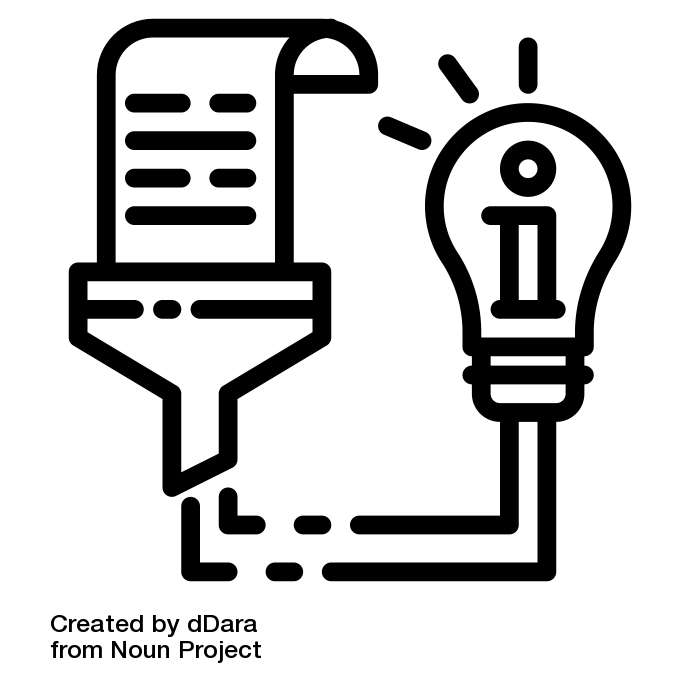
\includegraphics[width=0.9\textwidth]{../symbols/symbol_tex_content}
			\end{wrapfigure}
	

			\noindent Um neue Ölfelder zu finden, erkunden Unternehmen neue Regionen mit Testbohrungen. Auf diese Weise werden Gesteinsproben aus dem tiefen Erdinneren entnommen und können analysiert werden. Wenn eine der Bohrungen etwas Öl findet, besteht eine gute Chance, dass es ein riesiges Ölfeld zu fördern gibt. Nun entsteht an dieser Stelle ein Wald von Bohrstationen, bis eines Tages Öl aus einer der Bohrstationen herausschießt. Anschließend ersetzen Pumpen die Bohrer und pumpen Tag und Nacht Öl hoch. Am Anfang ist der Druck im Inneren des Ölfeldes groß genug, um das Öl an die Oberfläche zu drücken. Aber irgendwann nimmt der Druck ab. Wasser und andere Chemikalien werden in das Gestein gepumpt, um das Öl herauszupressen. Über Pipelines wird das Öl zu Raffinerien oder Häfen geschickt, wo es an Bord von riesigen Tankschiffen verladen und in die ganze Welt transportiert wird.
	

		\end{tcolorbox}

		\section{Raffinerie}
		
			\noindent \textbf{Auftrag: Erkläre wie Roh-Öl für die alltägliche Verwendung aufgearbeitet wird!}
			\begin{enumerate}
				\item \textbf{Lies} den Text und fasse die wichtigsten Punkte zusammen!
			\end{enumerate}

			\begin{tcolorbox}[enhanced,
				colback=white,
				colframe=darkgray,
				fonttitle=\sffamily\bfseries\large, 
				title=Erdölaufarbeitung,
				attach boxed title to top left={xshift=3.2mm,yshift=-0.50mm},
				boxed title style={skin=enhancedfirst jigsaw,height=0.7cm,size=small,arc=1mm,bottom=-1mm,colframe=darkgray,height=0.75cm},
				colbacktitle=darkgray,
				drop lifted shadow]
				\begin{wrapfigure}{L}{0.15\textwidth}  
					\centering
					\vspace{-14pt}  % to align image with first line of text
					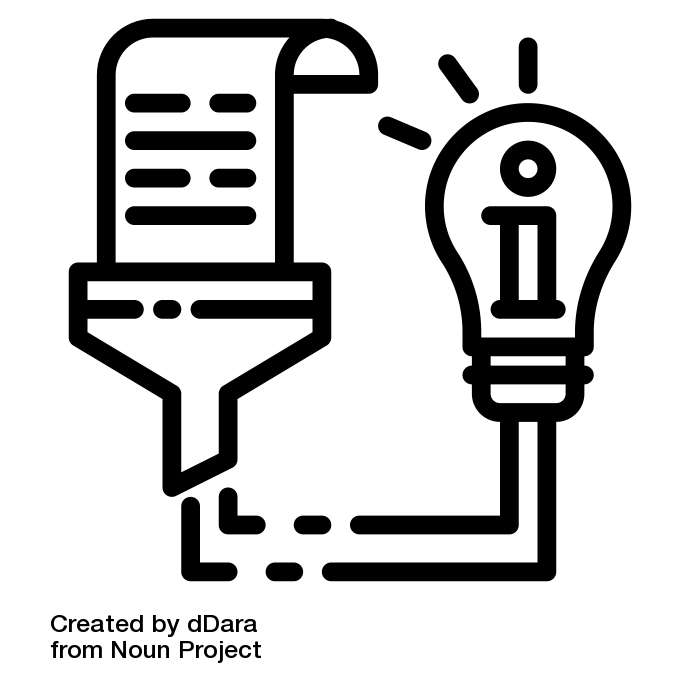
\includegraphics[width=0.9\textwidth]{../symbols/symbol_tex_content}
				\end{wrapfigure}
				
				
				\noindent Das Rohöl kann nicht sofort verwendet werden, da es mit Sand, Wasser, Salz und anderen Sedimenten verunreinigt ist. Öl zu raffinieren bedeutet, das Öl von diesen Stoffen zu reinigen. \newline
				Anschließend wird das Roh-Öl in einer fraktionierten Destillation in seine einzelnen Bestandteile getrennt.
				Die fraktionierte Destillation ist die häufigste Form der Trenntechnik, die in Erdölraffinerien eingesetzt wird. 
				Die industrielle Destillation wird normalerweise in großen, vertikalen zylindrischen Kolonnen durchgeführt, die als Destillations- oder Fraktionierungskolonnen mit Durchmessern von etwa 65 Zentimetern bis 6 Metern und Höhen von etwa 6 Metern bis 60 Metern oder mehr bekannt sind. Die Destillationstürme haben Flüssigkeitsauslässe in Abständen oberhalb der Kolonne, die die Entnahme von verschiedenen Fraktionen oder Produkten mit unterschiedlichen Siedepunkten oder Siedebereichen ermöglichen. Durch die Erhöhung der Temperatur des Produktes innerhalb der Kolonnen werden die verschiedenen Kohlenwasserstoffe getrennt. Die "leichtesten" Produkte (diejenigen mit dem niedrigsten Siedepunkt) treten am oberen Ende der Kolonnen aus, und die "schwersten" Produkte (diejenigen mit dem höchsten Siedepunkt) treten am unteren Ende der Kolonne aus.\footnote{Quelle (übersetzt und  angepasst): http://en.wikipedia.org/wiki/Fractional\_distillation}
			\end{tcolorbox}
\newpage
		\section{Zusammenfassung}
		
			\noindent \textbf{Auftrag: Erstelle in deinem Hefter eine Zusammenfassung!}
			\begin{enumerate}
				\item Übernimm die Abbildung in deinen Hefter\footnote{Quelle (angepasst): https://commons.wikimedia.org/wiki/File:Crude\_Oil\_Distillation-de.svg}.
				\item \textbf{Recherchiere} online und im Lehrbuch, welche Produkte bei den einzelnen Temperaturbereichen aus der Destillation gewonnen werden. Gib deine \textbf{Quellen} an!
				\item \textbf{Nenne} Verwendungsmöglichkeiten für die Produkte.
			\end{enumerate}
		
			\begin{figure}[h]
				\centering
				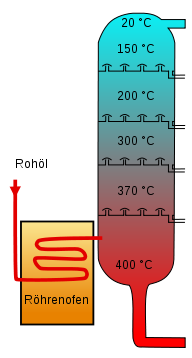
\includegraphics{img/crude_oil_distillation}
				\caption{Schematische Darstellung - Fraktionierte Destillation}
			\end{figure}


		\section{Destillation im Labor - Treibstoff für den Fluchtwagen}
			
			\textbf{Auftrag: Erläutere, wie du eine fraktionierte Destillation im Labor durchführen kannst.}
			\begin{enumerate}
				\item \textbf{Recherchiere}, welche Geräte man für eine (fraktionierte) Destillation benötigt. Gib deine \textbf{Quellen} an!
				\item \textbf{Recherchiere und erläutere} mit Hilfe einer Zeichnung, wie man die Destillation im Labor durchführt. Gib deine \textbf{Quellen} an!
				\item \textbf{Tipp:} In vielen Schule gibt es immer etwas Erdöl als Anschauungsobjekt und viele Glasgeräte, die man benutzen kann.
			\end{enumerate}
	

\end{document}

